\subsubsection{Remote Procedure Call}

Die Remote Procedure Call (RPC) Architektur ist ein Kommunikationsmodell, das es ermöglicht, Prozeduraufrufe zwischen Prozessen auf unterschiedlichen Systemen oder Maschinen durchzuführen. Die Idee hinter RPC besteht darin, entfernte Funktionen oder Methoden so einfach aufrufen zu können, als wären sie lokale Funktionen innerhalb des aufrufenden Programms.
\\\\
Aufbau einer RPC-Architektur:
\begin{itemize} 
\item Client: Der Client ist der Prozess oder die Anwendung, die den entfernten Prozeduraufruf initiiert. Der Client stellt eine Anfrage an den Server, um eine bestimmte Funktion auszuführen, und wartet auf die Antwort.
\item Client Stub: Der Client Stub ist eine lokale Repräsentation der entfernten Prozedur auf der Clientseite. Er ist dafür verantwortlich, die Anfrage des Clients in ein geeignetes Format umzuwandeln, das vom Server verstanden werden kann. Dieser Vorgang wird als \enquote{Marshalling} bezeichnet.
\item Kommunikationsprotokoll: Ein Kommunikationsprotokoll wird verwendet, um die Anfrage und die Antwort zwischen Client und Server zu übertragen. Dies kann beispielsweise ein TCP/IP- oder UDP-Protokoll sein, je nach den Anforderungen an Zuverlässigkeit, Geschwindigkeit und Latenz.
\item Server: Der Server ist der Prozess oder die Anwendung, die die angeforderte Funktion oder Methode bereitstellt. Der Server empfängt die Anfrage vom Client, führt die entsprechende Prozedur aus und sendet die Antwort zurück.
\item Server Stub: Der Server Stub empfängt die Anfrage vom Client, wandelt sie in ein für die Serverumgebung geeignetes Format um (\enquote{Unmarshalling}) und ruft die gewünschte Funktion auf. Anschließend werden die Ergebnisse wieder \enquote{gemarshalled} und an den Client gesendet.
\end{itemize}     

Im Folgenden wird der grundsätzliche Ablauf in einer RPC Architektur beschrieben, welcher noch verfeinert werden sollte, aber bereits die grundlegende Idee transportiert. 

\begin{enumerate} 
\item Der Client ruft die entfernte Prozedur über den Client Stub auf, als wäre es eine lokale Funktion.
\item Der Client Stub wandelt die Parameter der Anfrage in ein standardisiertes Format um (Marshalling) und sendet die Anfrage über das Kommunikationsprotokoll an den Server.
\item Der Server Stub empfängt die Anfrage, demarshalled die Parameter und ruft die entsprechende Funktion auf dem Server auf.
\item Die Funktion wird auf dem Server ausgeführt, und das Ergebnis wird an den Server Stub zurückgegeben.
\item Der Server Stub marshallt das Ergebnis und sendet es über das Kommunikationsprotokoll an den Client Stub zurück.
\item Der Client Stub empfängt die Antwort, demarshalled das Ergebnis und gibt es an den Client zurück.
\end{enumerate}

In einer RPC-Architektur kann die Kommunikation sowohl synchron als auch asynchron erfolgen. Bei synchroner Kommunikation wartet der Client auf die Antwort vom Server, bevor er weitere Aktionen ausführt. Dies kann zu Wartezeiten führen, insbesondere bei langsamen Netzwerkverbindungen oder komplexen Anfragen. Bei asynchroner Kommunikation sendet der Client die Anfrage und führt sofort weitere Aufgaben aus, ohne auf die Antwort zu warten. Die Antwort wird in der Regel über einen Callback-Mechanismus oder ein Event-System verarbeitet, sobald sie verfügbar ist.

Die RPC-Architektur ist in verschiedenen Anwendungen und Umgebungen weit verbreitet, wie z.B. bei verteilten Systemen, Client-Server-Anwendungen und Microservices. Sie bietet eine abstrakte und einfach zu verwendende Schnittstelle für die Kommunikation zwischen Prozessen auf verschiedenen Systemen, ohne dass sich der Entwickler um die Details der Netzwerkkommunikation kümmern muss.

Das Diagramm~\ref{fig:simple-rpc} zeigt einen ersten naiven Entwurf einer RPC Schichtenarchitektur. In diesem Ansatz existiert eine Schicht \enquote{Application}, welche die Schicht der Middleware nutzt, welche wiederum die Ressourcen - beispielhaft des Betriebssystems - nutzt, um die Kommunikation mittels Netzwerkprotokolle zu realisieren. 

\begin{figure}[!ht]
  \centering
  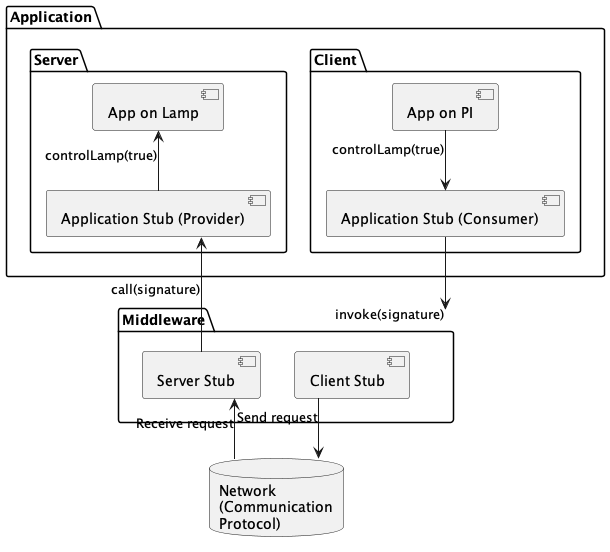
\includegraphics[width=0.95\textwidth]{fig/uml/rpc-simple.png}
  \caption{Erster Ansatz einer RPC Architektur}
  \label{fig:simple-rpc}
\end{figure}

Interessant ist die Einbringung einer zusätzlichen Schicht in der Applikation, die als Application Stub bezeichnet ist. Die Idee des Application-Stubs (auch als \enquote{Applikations-Stub} oder \enquote{App-Stub} bezeichnet) wurde von Andrew S. Tanenbaum entwickelt, um die Kommunikation und Interaktion zwischen Anwendungen und Middleware in verteilten Systemen zu erleichtern. Der Application-Stub ist eine Schnittstelle, die als Vermittler zwischen der Anwendung und der Middleware fungiert, um die Kommunikation und Zusammenarbeit zwischen diesen beiden Ebenen zu ermöglichen.

Die Umsetzung des Application-Stubs basiert auf der Trennung der Anwendungslogik von der Middleware-Kommunikationslogik. Dies wird erreicht, indem der Stub die Anwendungslogik von den Netzwerkdetails, wie z.B. den Marshalling/Unmarshalling von Daten, dem Verbindungsaufbau und dem Senden/Empfangen von Nachrichten, entkoppelt.

Um den Application-Stub in einer verteilten Umgebung zu nutzen, sind folgende Schritte erforderlich:
\begin{itemize} 
\item Entwurf einer Schnittstellenbeschreibung: Zunächst wird eine Schnittstellenbeschreibung erstellt, die die Funktionen und Methoden definiert, die von der Anwendung und der Middleware bereitgestellt werden sollen. Diese Schnittstellenbeschreibung kann in einer Interface Definition Language (IDL) oder einer ähnlichen Sprache definiert werden.
\item Erstellung des Application-Stubs: Basierend auf der Schnittstellenbeschreibung wird ein Application-Stub generiert oder manuell erstellt. Dieser Stub enthält Code, der die Kommunikation zwischen der Anwendung und der Middleware verwaltet. Es kann für verschiedene Programmiersprachen und Plattformen erstellt werden, um die Interoperabilität zu gewährleisten.
\item Integration des Application-Stubs in die Anwendung: Der generierte oder erstellte Application-Stub wird in die Anwendung integriert, indem er die definierten Funktionen und Methoden für die Kommunikation mit der Middleware implementiert. Die Anwendung ruft die Funktionen und Methoden des Stubs auf, als wären sie lokale Funktionen oder Methoden, ohne sich um die zugrunde liegenden Netzwerkdetails kümmern zu müssen. Das Factory Pattern kann hier eine Lösung sein, die Wahl zu implementieren.
\item Anpassung der Middleware: Die Middleware muss in der Lage sein, die Anfragen des Application-Stubs zu verarbeiten und entsprechend zu reagieren. Dies kann durch die Implementierung von Server-Stubs und der entsprechenden Kommunikationslogik erreicht werden.
\item Kommunikation zwischen Anwendung und Middleware: Durch die Verwendung des Application-Stubs kann die Anwendung nun nahtlos mit der Middleware kommunizieren, ohne sich um die Details der Netzwerkkommunikation kümmern zu müssen. Die Middleware empfängt die Anfragen, verarbeitet sie und sendet die Ergebnisse zurück an die Anwendung über den Application-Stub.
\end{itemize} 
Die Verwendung eines Application-Stubs bietet mehrere Vorteile, wie z.B.:
\begin{itemize} 
\item Entkopplung der Anwendungslogik von der Middleware-Kommunikationslogik, was zu einer besseren Trennung von Verantwortlichkeiten und einfacherer Wartung führt.
\item Vereinfachung der Kommunikation zwischen Anwendung und Middleware durch Abstraktion der Netzwerkdetails, sodass sich Entwickler auf die Anwendungslogik konzentrieren können.
\item Erhöhung der Interoperabilität zwischen Anwendungen und Middleware, da der Application-Stub in verschiedenen Programmiersprachen und Plattformen implementiert werden kann.
\item Verbesserung der Modularität und Skalierbarkeit von verteilten Systemen, da Anwendungen und Middleware unabhängig voneinander entwickelt, aktualisiert und erweitert werden können.
\end{itemize} 

Der Application-Stub ermöglicht nach Tanenbaum eine effiziente Kommunikation und Zusammenarbeit zwischen Anwendungen und Middleware in verteilten Systemen. Durch die Entkopplung der Anwendungslogik von der Kommunikationslogik können Entwickler sich auf die wesentlichen Aspekte der Anwendung konzentrieren, während die Middleware die Netzwerkkommunikation und andere Details verwaltet.
\\\\
Hier ist ein einfaches Beispiel in Java, das die Idee des Application-Stubs und das Factory-Pattern verwendet, um eine Anwendung mit Middleware zu verbinden. In diesem Beispiel simulieren wir eine einfache Lampe und ihre Steuerung.
Zuerst erstellen wir eine Lamp-Schnittstelle, die als Middleware fungiert:\\
\noindent\begin{minipage}{\textwidth}
\begin{lstlisting}[caption={RPC Interface},captionpos=b,label={lst:rpc-interface}]
public interface Lamp {
    void controlLamp(Boolean b);
}
\end{lstlisting}
\end{minipage}
Als nächstes erstellen wir eine Implementierung der Lamp-Schnittstelle auf dem Server-Anteil des Applikationscodes:\\

\noindent\begin{minipage}{\textwidth}
\begin{lstlisting}[caption={RPC Remote Implementation},captionpos=b,label={lst:rpc-remote}]
public class LampRemote implements Lamp {
    @Override
    public void controlLamp(boolean b){
    	List<Boolean> list = new ArrayList<Boolean>(); 
        Collections.addAll(list, b);
        Middleware.invoke("controlLamp", list);
    }
}
\end{lstlisting}
\end{minipage}
Nun erstellen wir eine Factory-Klasse, die als Application-Stub fungiert:\\
\noindent\begin{minipage}{\textwidth}
\begin{lstlisting}[caption={Application Stub mit Factory Pattern},captionpos=b,label={lst:rpc-factory}]
public class LampFactory {
    public static Lamp createLamp() {
        // Hier koennte die Middleware-Verbindung hergestellt werden.
        // In diesem Beispiel verwenden wir eine einfache lokale Implementierung.
        return new LampRemote();
    }
}
\end{lstlisting}
\end{minipage}
Schließlich erstellen wir eine Anwendungsklasse, die die Lamp-Schnittstelle verwendet:\\
\noindent\begin{minipage}{\textwidth}
\begin{lstlisting}[caption={Controller ruft Middleware},captionpos=b,label={lst:rpc-controller}]
public class LampController {
	public static void main(String[] args) {
        // Erstelle eine Lampe ueber die Factory-Methode (Application-Stub)
        Lamp lamp = LampFactory.createLamp();

        // Verwende die Lampe in der Anwendung
        lamp.controlLamp(true);
    }
}
\end{lstlisting}
\end{minipage}
In diesem Beispiel wurde eine Lamp-Schnittstelle erstellt, die als Middleware fungiert, um eine Lampe zu steuern. Die LampFactory-Klasse dient als Application-Stub, der die Erstellung und Verbindung zur Middleware verwaltet. Die Lamp Controller-Anwendung verwendet die Lamp-Schnittstelle über die Factory-Methode, um die Lampe ein- und auszuschalten.

In einer realen Anwendung könnte die LampFactory-Klasse die Verbindung zu einer tatsächlichen Middleware herstellen, anstatt einfach eine lokale Implementierung zu erstellen. Natürlich ist die Annahme einer Objektmenge nur aus dem Datentyp Boolean naiv, zeigt aber die Funktionsweise ausreichend auf. Die Anwendung selbst muss sich jedoch nicht um diese Details kümmern, da der Application-Stub diese Verantwortung übernimmt.

Diese zunächst einfache und naive Darstellung ist als Möglichkeit gedacht, um zunächst einen Überblick zu schaffen. Natürlich müssen hier verschiedene Aspekte verfeinert und für das bessere Verständnis nochmal diskutiert werden. 

Als erstes muss man festhalten, dass aus der naiven Ansicht häufig ein Verhalten abgeleitet wird, welches aber auf einer missverstandenen Interpretation der Architektur zurückzuführen ist, weniger auf ein noch nicht eingeführtes Verhaltensdiagramm. 
\\\\
Ist die Beschreibung des Verhaltens in der Architektur das Ziel, muss nochmals auf die Nutzung des Schichtenmodells hingewiesen werden. Jede Schicht kapselt die Sequenzen nach der zugeordneten Verantwortlichkeit.
Somit beschreiben die Sequenzen in der Applikationsschicht die der Applikation und die Sequenzen der Middleware die der Middleware. Was nicht geschehen sollte, ist eine Vermischung beider Schichten. So wäre eine gültige Sequenz der Applikation beschrieben in Diagramm~\ref{fig:rpc-app-seq-rpc} und eine der Middleware im Diagramm~\ref{fig:rpc-middleware-seq-rpc}. An der Sequenz in der Applikation selbst sollte man nicht ohne weiteres erkennen, dass es sich um einen entfernen Funktionsaufruf handelt. Diese Aufgabe wird von der Middleware übernommen.
\\\\
Es ist wichtig zu verstehen, dass die Sequenz der Applikation aus einer spezifischen Verarbeitung des Anwendungsfalls getrieben ist, wohingegen die Sequenz der Middleware eine generische Umsetzung repräsentiert, die von jeglichem Aufruf aus der Applikation heraus genutzt werden kann. So kann man naiv die Beziehung zwischen einem entfernten Funktionsaufruf und der Middleware auch als eine 0:n- Beziehung beschreiben, wobei die Middleware  in diesem Fall eine generische Funktion für einen synchronen Funktionsaufruf repräsentiert. 


 \begin{figure}[!ht]
  \centering
  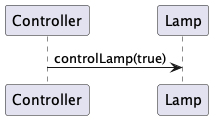
\includegraphics[width=0.30\textwidth]{fig/uml/rpc-app-seq.png}
  \caption{Beispielsequenz der App in der RPC Architektur}
  \label{fig:rpc-app-seq-rpc}
\end{figure}


 \begin{figure}[!ht]
  \centering
  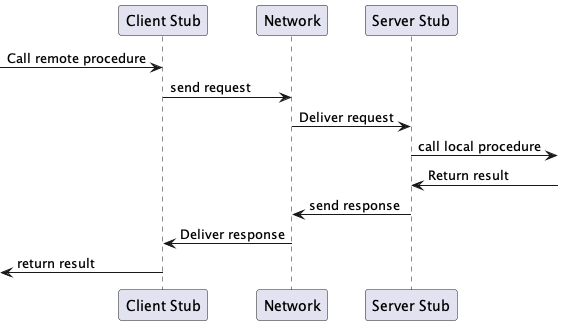
\includegraphics[width=0.65\textwidth]{fig/uml/rpc-middleware-seq.png}
  \caption{Beispielsequenz der Middleware in der RPC Architektur}
  \label{fig:rpc-middleware-seq-rpc}
\end{figure}

Um die Middleware möglichst transparent und wiederverwendbar zu gestalten, soll der Marshalling-Prozess genauer betrachtet werden, der im Client-Stub und Server-Stub eine besondere Rolle spielt, bevor die Nachrichten für den entfernten Funktionsaufruf versendet werden. 

Der Marshalling-Prozess und die Serialisierung sind Begriffe, die oft im Zusammenhang mit der Remote Procedure Call (RPC) Architektur verwendet werden. Beide Prozesse sind zwar miteinander verknüpft, es gibt jedoch grundlegende Unterschiede zwischen ihnen.
\\\\
Der Marshalling-Prozess ist ein Verfahren, bei dem Daten und Parameter in einer Form gewandelt werden, die über das Netzwerk gesendet und auf der anderen Seite wieder zusammengesetzt werden kann. Kurz: aus einem Funktionsaufruf wird eine Nachricht generiert. Dieser Prozess ist in der RPC-Architektur besonders wichtig, da hierdurch entfernte Prozeduraufrufe zwischen verschiedenen Systemen mit unterschiedlichen Datenformaten, Speicherlayouts oder sogar Programmiersprachen umgesetzt werden können.
\\\\
Der Marshalling-Prozess besteht aus mehreren Schritten:
\begin{itemize} 
\item Umwandlung der Daten und Parameter in ein plattformunabhängiges Format, oft in Form von Byte-Arrays.
\item Anfügen von Metadaten, wie zum Beispiel Typinformationen, um den Empfänger darüber zu informieren, wie die Daten wiederhergestellt werden können.
\item Zusammenpacken (Packing) der Daten und Metadaten in einer Nachricht, die über das Netzwerk gesendet werden kann.
\end{itemize} 

Die Serialisierung ist der Prozess der Umwandlung eines Objekts oder einer Datenstruktur in eine lineare, sequenzielle Darstellung, die zum Speichern oder Übertragen über ein Netzwerk verwendet werden kann. Serialisierung ist ein wichtiger Teil des Marshalling-Prozesses, da sie die Daten in eine übertragbare Form konvertiert. Sie ermöglicht es, den Zustand eines Objekts oder einer Datenstruktur zu erhalten, sodass es auf der Empfängerseite wiederhergestellt und verwendet werden kann. Unterschiede zwischen Marshalling und Serialisierung:
\begin{itemize} 
\item Anwendungsbereich: Serialisierung ist ein generischer Prozess, der nicht nur in der RPC-Architektur, sondern auch in anderen Anwendungen wie der persistenten Speicherung von Objekten und der Interprozesskommunikation verwendet wird. Marshalling ist spezifisch für die RPC-Architektur und bezieht sich auf das Vorbereiten von Daten und Parametern für entfernte Prozeduraufrufe.
\item Metadaten: Marshalling beinhaltet das Hinzufügen von Metadaten, die zur Interpretation und Rekonstruktion der übertragenen Daten auf der Empfängerseite erforderlich sind. Bei der Serialisierung werden hauptsächlich die Daten selbst in eine sequenzielle Darstellung umgewandelt, ohne notwendigerweise zusätzliche Metadaten hinzuzufügen.
\end{itemize} 
Im Weiteren soll ein Beispiel für einen Marshalling-Prozess ausgearbeitet werden. Angenommen, es gibt zwei Systeme A und B, die unterschiedliche Programmiersprachen und Datenformate verwenden. System A möchte eine Funktion auf System B aufrufen, die zwei Parameter akzeptiert: einen String und einen Integer. Der Marshalling-Prozess auf System A würde wie folgt aussehen:
\begin{itemize} 
\item Konvertierung der Parameter (z.B. String und Integer) in ein plattformunabhängiges Format, z. B. Byte-Arrays.
\item Hinzufügen von Metadaten, wie Typinformationen, zur Identifizierung der Parameter auf der Empfängerseite.
\item Zusammenpacken der Byte-Arrays und Metadaten in einer Nachricht, die über das Netzwerk gesendet werden kann
\end{itemize} 

Das Ziel, den Marshalling Process möglich generisch zu gestallten, ist in dem Prinzip \enquote{Copy in, Copy out} zusammengefasst. Der Begriff \enquote{Copy in, Copy out} (auch als \enquote{Call by Value-Result} bezeichnet) ist eine Semantik zur Übergabe von Parametern bei entfernten Prozeduraufrufen (RPCs) oder in Programmiersprachen. Es beschreibt die Art und Weise, wie Daten und Parameter zwischen dem aufrufenden und dem aufgerufenen System übertragen werden. Hier ist das grundlegende Prinzip von \enquote{Copy in, Copy out}:
\begin{itemize} 
\item Copy in: Beim Aufruf einer entfernten Funktion kopiert das aufrufende System die Werte der Parameter in eine Nachricht, die an das aufgerufene System gesendet wird. Dieser Schritt beinhaltet den Marshalling-Prozess, bei dem die Parameter in ein plattformunabhängiges Format konvertiert und Metadaten hinzugefügt werden.
\item Copy out: Nachdem die entfernte Funktion auf dem aufgerufenen System ausgeführt wurde, werden die Ergebnisse (Rückgabewerte oder geänderte Parameter) zurück zum aufrufenden System gesendet. Der Rückgabewert und die geänderten Parameter durchlaufen den Marshalling-Prozess erneut, um sie in eine übertragbare Form zu bringen. Anschließend kopiert das aufrufende System die empfangenen Daten in die ursprünglichen Variablen oder Speicherbereiche.
\end{itemize} 
\enquote{Copy in, Copy out} bietet einige Vorteile: Es vermeidet die direkte Manipulation von Speicheradressen zwischen unterschiedlichen Systemen, was bei verteilten Systemen mit unterschiedlichen Speicherlayouts und Adressräumen problematisch sein kann. Weiterhin stellt es sicher, dass das aufgerufene System nur auf Kopien der übergebenen Daten arbeitet, wodurch Seiteneffekte und unerwartete Änderungen der Daten auf dem aufrufenden System vermieden werden. Zuletzt erlaubt es die Verwendung verschiedener Programmiersprachen und Datenformate auf dem aufrufenden und aufgerufenen System, da die Daten beim Marshalling in ein plattformunabhängiges Format konvertiert werden.

Ein Nachteil von \enquote{Copy in, Copy out} ist jedoch der zusätzliche Overhead, der durch das Kopieren und Marshalling/Unmarshalling der Daten entsteht. Dies kann die Leistung und Effizienz des entfernten Prozeduraufrufs beeinträchtigen, insbesondere bei großen Datenmengen oder komplexen Datenstrukturen. In solchen Fällen können andere Parameterübergabemechanismen, wie beispielsweise \enquote{Call by Reference}, in Betracht gezogen werden, bei denen nur die Speicheradressen der Daten übertragen werden und somit der Overhead reduziert wird. 

Allerdings bringt dies auch zusätzliche Herausforderungen und Risiken mit sich, wie zum Beispiel die Notwendigkeit, die unterschiedlichen Adressräume der beteiligten Systeme zu verwalten, und das Risiko unerwarteter Seiteneffekte, wenn das aufgerufene System direkt auf den Speicher des aufrufenden Systems zugreift.

Um den Overhead bei der Verwendung von \enquote{Copy in, Copy out} zu minimieren, können verschiedene Optimierungen angewendet werden, wie zum Beispiel:

\begin{itemize} 
\item Datenkompression: Durch die Komprimierung der Daten während des Mar-shalling-Prozesses kann die Menge der übertragenen Daten reduziert werden, was zu einer schnelleren Übertragung und geringeren Netzwerkbelastung führt.
\item Verwendung effizienter Serialisierungsformate: Einige Serialisierungsformate, wie beispielsweise Protocol Buffers oder MessagePack, sind darauf ausgelegt, Daten effizienter und kompakter zu übertragen als textbasierte Formate wie JSON oder XML.
\item Selektive Übertragung: In einigen Fällen ist es möglich, nur die notwendigen Teile einer Datenstruktur oder eines Objekts zu übertragen, anstatt das gesamte Objekt zu kopieren und zu übertragen. Dies kann den Overhead der Parameterübergabe reduzieren.
\end{itemize} 

Bei der Verwendung von \enquote{Copy in, Copy out} in der RPC-Architektur ist es wichtig, die Datentypen der Parameter und Rückgabewerte korrekt zu bestimmen, um eine erfolgreiche Kommunikation zwischen dem aufrufenden und dem aufgerufenen System zu gewährleisten. 

Mit der \enquote{Copy in, Copy out} Semantik können Prozesse automatisiert werden, um die Codeanteile in einer RPC-Middleware zu bestimmen. Diese automatisierte Code-Generierung kann in folgende Schritte durchgeführt werden:
\begin{itemize} 
\item Definieren der Schnittstellen und Datenstrukturen, die in den entfernten Prozeduraufrufen verwendet werden. Dies geschieht mittels einer Interface Definition Language (IDL). Die IDL beschreibt die Signatur der entfernten Funktionen, einschließlich der Datentypen der Parameter und Rückgabewerte
\item Generieren des Stub- und Skeleton-Codes aus der IDL-Definition. Die meisten RPC-Middleware-Tools bieten Code-Generatoren an, die aus der IDL-Definition automatisch Stub- und Skeleton-Code für verschiedene Programmiersprachen erstellen. Der Stub-Code dient als Proxy für den Aufrufer, während der Skeleton-Code die Implementierung der entfernten Funktion auf dem aufgerufenen System kapselt. Beide Teile des Codes enthalten die notwendigen Informationen über die Datentypen für das Marshalling und Unmarshalling der Daten.
\item Implementierung der entfernten Funktionen auf dem aufgerufenen System unter Verwendung des generierten Skeleton-Codes. Dies stellt sicher, dass die Implementierung der Funktionen mit den in der IDL-Definition angegebenen Datentypen übereinstimmt.
\item  Verwendung des generierten Stub-Codes auf dem aufrufenden System, um entfernte Prozeduraufrufe durchzuführen. Der Stub-Code stellt sicher, dass die Parameter und Rückgabewerte korrekt gemarshalled und unmarshalled werden, basierend auf den in der IDL-Definition festgelegten Datentypen.
\end{itemize} 
Zentrale Komponente ist die  Interface Definition Language (IDL). Eine Interface Definition Language ist eine formale Beschreibungssprache, die verwendet wird, um Schnittstellen zwischen Softwarekomponenten und Diensten in einer standardisierten und plattformunabhängigen Weise zu definieren. Die Verwendung einer IDL in Verbindung mit einem Code-Generator bietet mehrere Vorteile für die automatische Erstellung von Remote Procedure Call Lösungen.

Ein Code-Generator für Interface Definition Language ist ein Software-Tool, das automatisch Code in einer oder mehreren Programmiersprachen auf der Grundlage einer IDL-Definition erstellt. Der Prozess der Codegenerierung aus einer IDL umfasst mehrere Schritte:
\begin{itemize} 
\item Analyse der IDL-Datei: Der Code-Generator liest und analysiert die IDL-Datei, die die Schnittstellendefinitionen, Funktionen, Datenstrukturen und Datentypen enthält, die für die Kommunikation zwischen den verschiedenen Komponenten eines verteilten Systems benötigt werden.
\item Parsen der IDL-Datei: Der Code-Generator verwendet einen Parser, um die IDL-Datei in einen abstrakten Syntaxbaum (AST) oder ein ähnliches internes Format zu zerlegen, dass leichter für die Codegenerierung verwendet werden kann.
\item Code-Generierung: Basierend auf dem internen Format erstellt der Code-Generator automatisch den notwendigen Client- und Server-Code für die Kommunikation über das verteilte System. Dies kann Stub- und Skeleton-Code für verschiedene Programmiersprachen umfassen, die für den Remote Procedure Call verwendet werden.
\item Sprachspezifische Anpassungen: Der Code-Generator berücksichtigt die Besonderheiten der jeweiligen Zielsprache, um sicherzustellen, dass der generierte Code den Konventionen und Syntaxanforderungen dieser Sprache entspricht. Dies umfasst die Anpassung von Datentypen, Namenskonventionen und anderen sprachspezifischen Details.
\item Code-Ausgabe: Schließlich gibt der Code-Generator den erstellten Code als Dateien aus, die in das Zielsystem integriert werden können. Dies ermöglicht Entwicklern, die generierten Stubs und Skeletons in ihrem Projekt zu verwenden, um die definierten Schnittstellen über RPC aufzurufen oder bereitzustellen.
\end{itemize} 

Aus diesen Schritten soll nun ein Beispiel abgeleitet werden, welches auch den manuellen Aufbau einer Lösung beschreibt. Angenommen, es gibt ein verteiltes System, in dem ein Client eine entfernte Funktion \enquote{add} aufrufen möchte, die zwei Integer-Parameter akzeptiert und einen Integer-Wert zurückgibt.

Zunächst wird eine Schnittstelle der entfernten Funktion in einer IDL definiert. \\
\noindent\begin{minipage}{\textwidth}
\begin{lstlisting}[caption={IDL Example},captionpos=b,label={lst:idl-example}]
interface MathService {
  int add(in int a, in int b);
}
\end{lstlisting}
\end{minipage}
Diese IDL-Definition beschreibt eine Schnittstelle namens \enquote{MathService} mit einer Funktion \enquote{add}, die zwei Integer-Parameter (\enquote{a} und \enquote{b}) akzeptiert und einen Integer-Wert zurückgibt.

Aus diesen Informationen kann ein  Stub- und Skeleton-Code generiert werden. Abhängig von der verwendeten RPC-Middleware und Programmiersprache erhalten Sie möglicherweise Klassen oder Module, die die \enquote{MathService}-Schnittstelle implementieren und die notwendigen Informationen über die Datentypen enthalten.

Danach ist die \enquote{add}-Funktion auf dem aufgerufenen System unter Verwendung des generierten Skeleton-Codes zu implementieren. So könnte eine Implementierung aussehen:\\
\noindent\begin{minipage}{\textwidth}
\begin{lstlisting}[caption={RPC IDL Service Impl},captionpos=b,label={lst:idl-impl}]
class MathServiceImpl(MathService):
    def add(self, a, b):
        return a + b
\end{lstlisting}
\end{minipage}
Nun kann der generierte Stub-Code auf dem aufrufenden System genutzt werden, um die \enquote{add}-Funktion über einen RPC-Aufruf aufzurufen.\\
\noindent\begin{minipage}{\textwidth}
\begin{lstlisting}[caption={RPC IDL Service Impl},captionpos=b,label={lst:idl-impl-service}]
math math_service_client = MathServiceStub(server_address)
result = math_service_client.add(5, 7)
print("Result of 5 + 7:", result)
\end{lstlisting}
\end{minipage}
In diesem Beispiel erstellen wir eine Instanz des MathServiceStub, der als Client für den entfernten MathService fungiert. Wir rufen die add-Funktion über den Stub auf und übergeben die Integer-Parameter 5 und 7. Der Stub kümmert sich um das Marshalling der Daten und das Senden der Anfrage an den entfernten Server. Der entfernte Server führt die Funktion add aus und sendet das Ergebnis (12) zurück zum Client. Der Stub verwaltet das Unmarshalling der Daten, und der Client erhält das korrekte Ergebnis.

Durch die korrekte Bestimmung der Datentypen und die Verwendung von IDL, Stub und Skeleton wird sichergestellt, dass die \enquote{Copy in, Copy out}-Semantik korrekt angewendet wird und die Kommunikation zwischen dem aufrufenden und dem aufgerufenen System erfolgreich ist. Zudem kann man sich durch gute Code Generatoren viel Arbeit ersparen. 

RPC-Lösungen wie XML-RPC und gRPC arbeiten auch nach dem \enquote{Copy in, Copy out}-Prinzip und nutzen die Marshalling/Unmarshalling-Techniken, um Daten zwischen den aufrufenden und aufgerufenen Systemen zu übertragen. 

XML-RPC ist eine RPC-Technik, die XML für die Kodierung von Daten und HTTP für die Datenübertragung verwendet. In diesem Beispiel implementieren wir einen einfachen Additionsdienst:

\noindent\begin{minipage}{\textwidth}
\begin{lstlisting}[caption={XML-RPC in Python},captionpos=b,label={lst:xmp-rpc-python}]
from xmlrpc.server import SimpleXMLRPCServer

def add(a, b):
    return a + b

server = SimpleXMLRPCServer(("localhost", 8080))
server.register_function(add, "add")
server.serve_forever()
\end{lstlisting}
\end{minipage}

In diesem Beispiel ist die \enquote{add}-Funktion auf dem Server registriert. Der Client verwendet einen Proxy, um die entfernte Funktion aufzurufen. Die Parameter (5 und 7) werden automatisch in XML kodiert (gemarshalled), und die Anfrage wird über HTTP an den Server gesendet. Der Server führt die Funktion aus und sendet das Ergebnis (12) zurück, das wiederum vom Client automatisch aus XML dekodiert (unmarshalled) wird.

Als alternative zu XML-RPC kann auch gRPC betrachtet werden. gRPC ist eine moderne, leistungsfähige RPC-Implementierung, die auf Protocol Buffers für die Datenkodierung und HTTP/2 für die Datenübertragung basiert. In diesem Beispiel implementieren wir denselben Additionsdienst wie im XML-RPC-Beispiel:

Zuerst definieren wir die Schnittstelle in einer Protocol Buffers IDL-Datei 

\noindent\begin{minipage}{\textwidth}
\begin{lstlisting}[caption={gRPC IDL},captionpos=b,label={lst:grpc-idl}]
syntax = "proto3";

service MathService {
  rpc Add(AddRequest) returns (AddResponse);
}

message AddRequest {
  int32 a = 1;
  int32 b = 2;
}

message AddResponse {
  int32 result = 1;
}
\end{lstlisting}
\end{minipage}

Weiter braucht es noch eine Implementierung der serverseitigen Funktion:

\noindent\begin{minipage}{\textwidth}
\begin{lstlisting}[caption={gRPC Server Python},captionpos=b,label={lst:grpc-server}]
import grpc
from concurrent import futures
import math_service_pb2
import math_service_pb2_grpc

class MathServiceImpl(math_service_pb2_grpc.MathServiceServicer):
    def Add(self, request, context):
        return math_service_pb2.AddResponse(result=request.a + request.b)

server = grpc.server(futures.ThreadPoolExecutor(max_workers=10))
math_service_pb2_grpc.add_MathServiceServicer_to_server(MathServiceImpl(), server)
server.add_insecure_port("[::]:8080")
server.start()
server.wait_for_termination()
\end{lstlisting}
\end{minipage}

\noindent\begin{minipage}{\textwidth}
\begin{lstlisting}[caption={gRPC Client Python},captionpos=b,label={lst:grpc-client}]
import grpc
import math_service_pb2
import math_service_pb2_grpc

channel = grpc.insecure_channel("localhost:8080")
stub = math_service_pb2_grpc.MathServiceStub(channel)
request = math_service_pb2.AddRequest(a=5, b=7)
response = stub.Add(request)
print("Result of 5 + 7:", response.result)
\end{lstlisting}
\end{minipage}

In diesem gRPC-Beispiel wird die Schnittstelle in einer Protocol Buffers IDL-Datei definiert. Der Server implementiert die Add-Funktion und registriert sie im gRPC-Server. Der Client erstellt einen Stub, um die entfernte Funktion aufzurufen. Die Anfrage- und Antwortdaten werden automatisch in Protocol Buffers kodiert (gemarshalled) und dekodiert (unmarshalled).

In beiden Beispielen (XML-RPC und gRPC) arbeiten die Lösungen nach dem \enquote{Copy in, Copy out}-Prinzip.

In der RPC (Remote Procedure Call) Terminologie beziehen sich die Begriffe Skeleton, Server-Stub und Server-Proxy auf verschiedene Aspekte der serverseitigen Implementierung, die in der Kommunikation zwischen Client und Server verwendet werden. 

\begin{itemize} 
\item Skeleton: Das Skeleton ist der serverseitige Code, der als Vermittler zwischen dem Netzwerk und der eigentlichen Implementierung der Serverfunktionalität fungiert. Es ist dafür verantwortlich, eingehende Anfragen zu empfangen, die über das Netzwerk gesendet werden, und diese in lokale Aufrufe der entsprechenden Methoden umzuwandeln. Das Skeleton nimmt die Ergebnisse dieser Methodenaufrufe entgegen, verpackt sie in eine Antwortnachricht und sendet sie zurück an den Client. In manchen Implementierungen ist das Skeleton identisch mit dem Server-Stub.
\item Server-Stub: Der Server-Stub ist der auf der Serverseite \enquote{generierte} Code, der die Kommunikation zwischen dem Client und der eigentlichen Implementierung der Serverfunktionalität erleichtert. Der Stub empfängt die Anfragen von den Clients, extrahiert die notwendigen Parameter aus der Nachricht und ruft die entsprechende Methode auf der Serverimplementierung auf. Nachdem die Methode ausgeführt wurde, verpackt der Stub das Ergebnis und sendet es zurück an den Client. In manchen Implementierungen ist der Server-Stub identisch mit dem Skeleton.
\item Server-Proxy: Ein Server-Proxy ist eine Art von Server-Stub oder Skeleton, der zusätzliche Funktionen wie Sicherheit, Lastverteilung oder Caching bereitstellen kann. Während ein einfacher Stub oder Skeleton hauptsächlich für die Übersetzung von Nachrichten und das Aufrufen von Methoden verantwortlich ist, kann ein Proxy zusätzliche Kontroll- oder Verwaltungsaufgaben übernehmen. Ein Server-Proxy kann beispielsweise Anfragen von mehreren Clients entgegennehmen und diese auf verschiedene Serverinstanzen verteilen, um die Last auszugleichen.
\end{itemize} 

Bevor das Kapitel um RPC abgeschlossen wird, soll nochmal ein verwandtes Thema zu RPC mit Remote Method Invocation (RMI)  aufgenommen werden. RPC und RMI sind zwei Techniken, die es ermöglichen, Methoden oder Prozeduren auf entfernten Systemen oder Prozessen aufzurufen. Beide Konzepte sind eng miteinander verbunden, aber es gibt einige Unterschiede in der Implementierung und den verfügbaren Funktionen.

\begin{itemize} 
\item Sprachunabhängigkeit: RPC ist eine sprachunabhängige Technik und kann in verschiedenen Programmiersprachen und Plattformen implementiert werden. RMI hingegen ist speziell für eine eine Objekt-orientierte Programmiersprache entwickelt worden und erfordert die Verwendung der gleichen Sprache (z.B. Java) auf beiden Seiten der Kommunikation (Client und Server).
\item Kommunikationsprotokoll: RPC verwendet in der Regel ein standardisiertes Protokoll wie HTTP, gRPC oder XML-RPC, um Anfragen und Antworten über das Netzwerk zu übertragen. RMI verwendet häufig properitäte Protokolle, wie das Java-RMI-Protokoll. Das Java-RMI-Protokoll basiert auf der Java-RMI-Wire-Protocol-Spezifikation  und ist speziell für die Übertragung von Java-Objekten entwickelt worden.
\end{itemize} 
Hier ist ein einfaches Java RMI-Beispiel, das einen Additionsdienst bereitstellt. Dieses Beispiel besteht aus zwei Teilen: dem Server und dem Client. Das gegebene Java RMI-Beispiel demonstriert, wie man einen  entfernten Dienst erstellt, der zwei Zahlen addiert. Hier ist der Hintergrund und die Erklärung für die verschiedenen Teile des Beispiels:
\\\\
Das Remote-Interface definiert die Methoden, die von entfernten Clients aufgerufen werden können. In diesem Fall gibt es eine einzige Methode add, die zwei Ganzzahlen als Parameter akzeptiert und ihre Summe als Ergebnis zurückgibt. Das Interface erweitert java.rmi.Remote, was erforderlich ist, um ein Interface als RMI-fähig zu kennzeichnen.

\noindent\begin{minipage}{\textwidth}
\begin{lstlisting}[caption={Remote-Interface (Calculator.java)},captionpos=b,label={lst:rmi-server}]
import java.rmi.Remote;
import java.rmi.RemoteException;

public interface Calculator extends Remote {
    int add(int x, int y) throws RemoteException;
}
\end{lstlisting}
\end{minipage}
Implementierung des Remote-Interfaces (CalculatorImpl.java):
Die CalculatorImpl-Klasse implementiert das Calculator-Interface und erweitert UnicastRemoteObject. Durch das Erweitern von UnicastRemoteObject wird die Implementierung automatisch exportiert, sodass sie von entfernten Clients aufgerufen werden kann.

\noindent\begin{minipage}{\textwidth}
\begin{lstlisting}[caption={Remote-Interface Implementierung (CalculatorImpl.java.java)},captionpos=b,label={lst:rmi-server}]
import java.rmi.RemoteException;
import java.rmi.server.UnicastRemoteObject;

public class CalculatorImpl extends UnicastRemoteObject implements Calculator {
    public CalculatorImpl() throws RemoteException {
    }

    @Override
    public int add(int x, int y) throws RemoteException {
        return x + y;
    }
}
\end{lstlisting}
\end{minipage}
Der RMI-Server ist für die Registrierung und Bereitstellung des entfernten Dienstes verantwortlich. Im Beispiel wird eine CalculatorImpl-Instanz erstellt, und die RMI-Registry wird gestartet, um den Dienst unter dem Namen \enquote{CalculatorService} zu veröffentlichen. Der Server wartet dann auf eingehende Client-Anfragen.

\noindent\begin{minipage}{\textwidth}
\begin{lstlisting}[caption={ RMI-Server (RMIServer.java)},captionpos=b,label={lst:rmi-server}]
import java.rmi.registry.LocateRegistry;
import java.rmi.registry.Registry;

public class RMIServer {
    public static void main(String[] args) {
        try {
            CalculatorImpl calculator = new CalculatorImpl();
            Registry registry = LocateRegistry.createRegistry(1099);
            registry.rebind("CalculatorService", calculator);
            System.out.println("CalculatorService is ready.");
        } catch (Exception e) {
            System.err.println("Server exception: " + e.toString());
            e.printStackTrace();
        }
    }
}
\end{lstlisting}
\end{minipage}
Der RMI-Client ist für das Herstellen einer Verbindung zum RMI-Server und das Aufrufen der entfernten Methoden verantwortlich. Im Beispiel wird der Client zunächst mit der RMI-Registry verbunden und holt dann den \enquote{CalculatorService} aus der Registry. Anschließend wird die add-Methode auf dem Remote-Dienst aufgerufen, um zwei Zahlen zu addieren, und das Ergebnis wird auf der Konsole ausgegeben.

\noindent\begin{minipage}{\textwidth}
\begin{lstlisting}[caption={ RMI-Client (RMIClient.java)},captionpos=b,label={lst:rmi-server}]
import java.rmi.registry.LocateRegistry;
import java.rmi.registry.Registry;

public class RMIClient {
    public static void main(String[] args) {
        try {
            Registry registry = LocateRegistry.getRegistry("localhost", 1099);
            Calculator calculatorService = (Calculator) registry.lookup("CalculatorService");
            int result = calculatorService.add(5, 3);
            System.out.println("5 + 3 = " + result);
        } catch (Exception e) {
            System.err.println("Client exception: " + e.toString());
            e.printStackTrace();
        }
    }
}
\end{lstlisting}
\end{minipage}
Das Beispiel illustriert die grundlegende Funktionsweise von Java RMI in verteilten Systemen. Mit RMI können Entwickler entfernte Objekte und Methodenaufrufe so behandeln, als wären sie lokale Objekte und Methoden, was die Entwicklung von verteilten Anwendungen vereinfacht.